\documentclass[11pt]{article} % use larger type; default would be 10pt

\usepackage[utf8]{inputenc}
\usepackage{geometry} % to change the page dimensions
\geometry{a4paper} % or letterpaper (US) or a5paper or....
\usepackage{graphicx} % support the \includegraphics command and options
\graphicspath{ {./foto/} }
\usepackage{booktabs} % for much better looking tables
\usepackage{array} % for better arrays (eg matrices) in maths
\usepackage{paralist} % very flexible & customisable lists (eg. enumerate/itemize, etc.)
\usepackage{verbatim} % adds environment for commenting out blocks of text & for better verbatim
\usepackage{subfig} % make it possible to include more than one captioned figure/table in a single float
% These packages are all incorporated in the memoir class to one degree or another...

%%% HEADERS & FOOTERS
\usepackage{fancyhdr} % This should be set AFTER setting up the page geometry
\pagestyle{fancy} % options: empty , plain , fancy
\renewcommand{\headrulewidth}{0pt} % customise the layout...
\lhead{}\chead{}\rhead{}
\lfoot{}\cfoot{\thepage}\rfoot{}

%%% SECTION TITLE APPEARANCE
\usepackage{sectsty}
\allsectionsfont{\sffamily\mdseries\upshape} % (See the fntguide.pdf for font help)
% (This matches ConTeXt defaults)

%%% ToC (table of contents) APPEARANCE
\usepackage[nottoc,notlof,notlot]{tocbibind} % Put the bibliography in the ToC
\usepackage[titles,subfigure]{tocloft} % Alter the style of the Table of Contents
\renewcommand{\cftsecfont}{\rmfamily\mdseries\upshape}
\renewcommand{\cftsecpagefont}{\rmfamily\mdseries\upshape} % No bold!

%%% END Article customizations


\title{Navodila za uporabo portala Pišek}
\author{Špenko Krištof, Flajs Žiga, Dobravec Blaž}
%\date{} % Activate to display a given date or no date (if empty),
         % otherwise the current date is printed 

\begin{document}
\maketitle

\pagebreak
\tableofcontents
\pagebreak
%__________________________________________________Osnovno
\section{Osnovno}

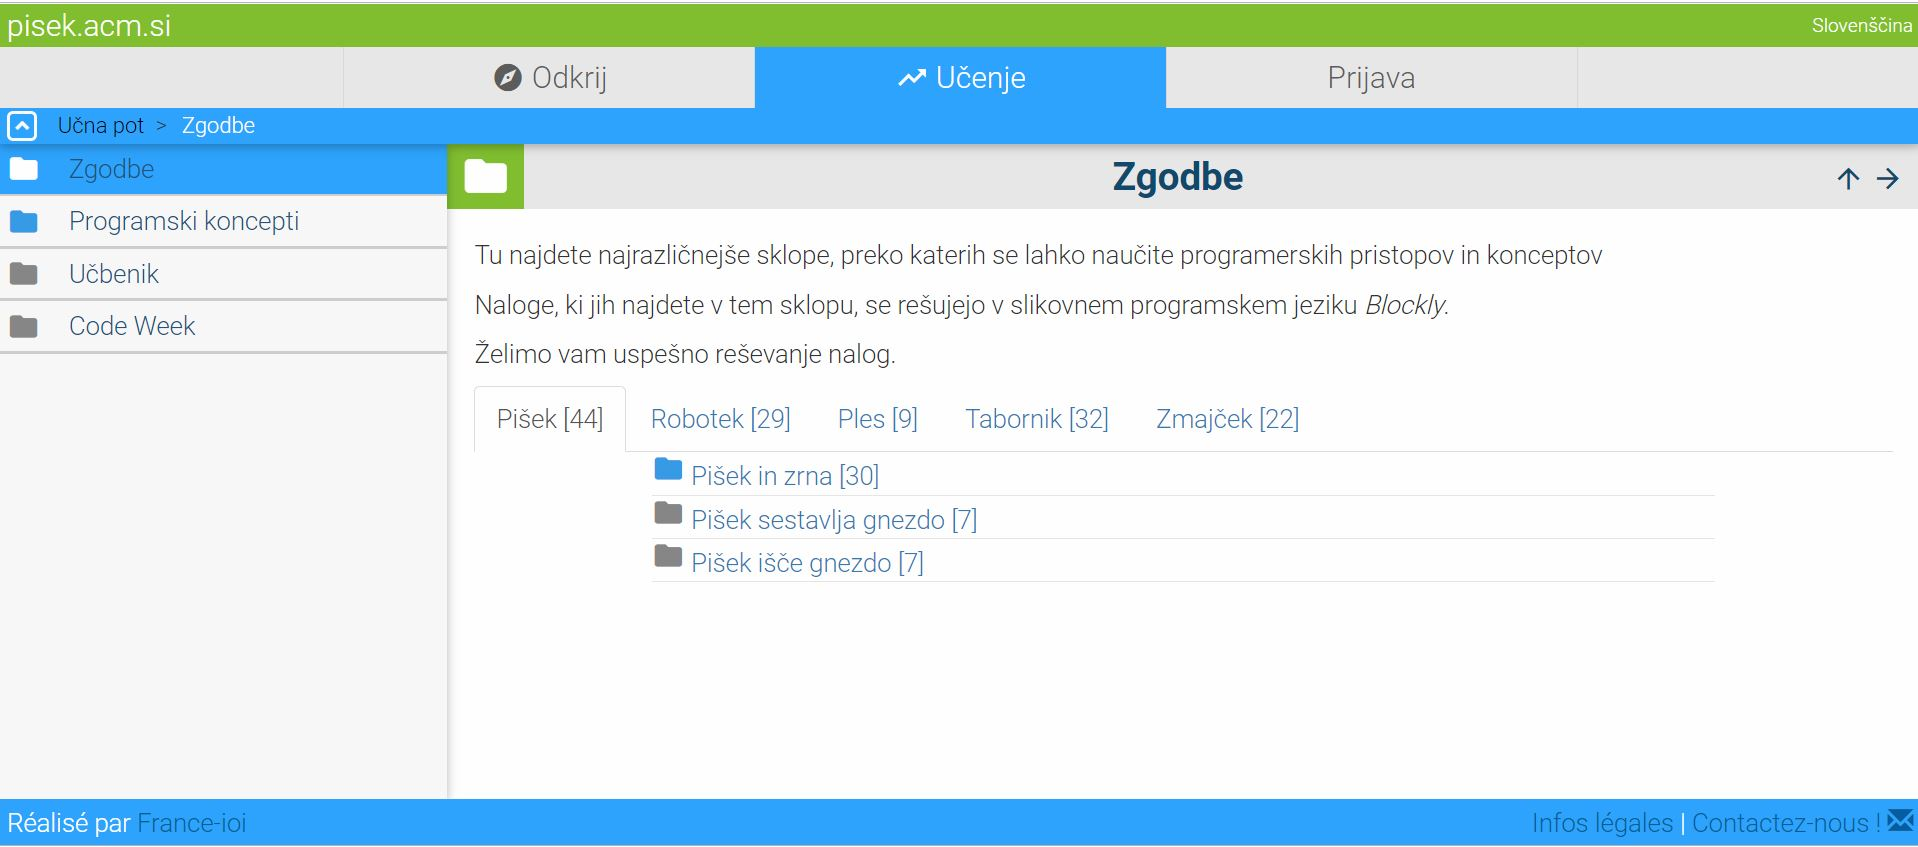
\includegraphics[width=\textwidth]{Portal_stran}

Portal je v osnovi razdeljen na različne sklope:
\begin{itemize}
\item Zgodbe
\item Programski koncepti
\item Učbenik
\item Code Week
\end{itemize}

V vsakem od sklopov so različne naloge, vendar \textbf{POZOR} v sklopu \textit{Zgodbe} in sklopu \textit{Učbenik} so naloge originalne, v \textbf{vseh} ostalih sklopih pa so naloge le kopije teh iz Učbenika in Zgodb.\\

V zavihku Odkrij oz. Navodila se nahaja text, kjer je opisano kako je nastal portal Pišek in podrobnosti, kontakt/ financiranje ipd.\\
To se ureja na SVN na naslovu:
\begin{center}
..\textbackslash Slovenia\textbackslash Ostalo\textbackslash Navodila\textbackslash index.html
\end{center}

\pagebreak
%__________________________________________________Izdelava nove naloge
\section{Izdelava nove naloge}

\subsection{Splošna navodila}

Ta del se nanaša na vse tipe nalog, torej so neka splošna navodila, kjer se obravnava stvari, ki so skupne vsem nalogam. razloži se tudi neke splošno razdelavo posamezne datoteke.\\

V mapi na SVN repozitoriju, kjer se nahaja naloga, so naslednje datoteke:
\begin{itemize}
\item \textit{$index.html$}
\item \textit{$taks.js$}
\item Knjižnica z lastnostmi posamezne datoteke (ta del je začasen, saj bi bilo v prihodnosti bolje, da so te datoteke definirane samo na enem mestu.), ki so pomenovane: \textit{blocklyRobot\textunderscore lib.js} ali \textit{blocklyPrinter\textunderscore lib.js} ali \textit{blocklyTurtle\textunderscore lib.js} ta datoteka je ustrezno poimenovana, v primeru da smo v zgodbi Tabornik, se tudi datoteka imenuje: \textit{blocklyTabornik\textunderscore lib.js}
\item v primeru, da ima naloga vključene fotografije, se le te prav tako nahajajo tukaj
\end{itemize}

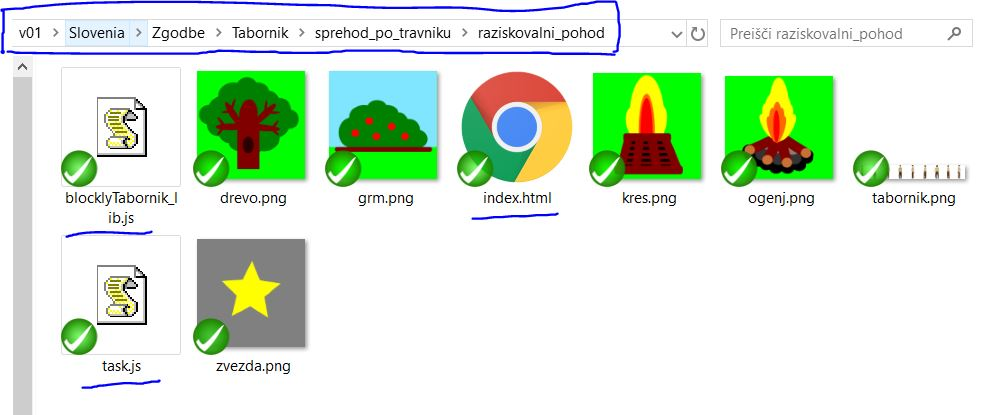
\includegraphics[scale=0.4]{svn_naloga}
%%%%%%%%%%%%%%%%%%%%%%%%%%%%%%%%%%%%%%%%%%%%%%%%%%%%%%%%%%%%%%%%%%%%%%%%%%%%%%%%%%%%%%%%%%%%%%%%%%%%%%%%%%%%%%%%%INDEX-SPLOŠNO
\subsubsection{index}

Ta datoteka se uporablja predvsem za to, da postavimo ogrodje samega izgleda, oziroma, da zloži vse komponente v neko celoto. \\[0.5cm]
V tej datoteki se napiše tudi besedilo vsake od podnalog. Obenem pa se znotraj te datoteke vključi vse potrebne module, prav tako lahko tu vključimo kakšne nove module, ki bodo dostopni v prihodnosti. \\[0.5cm]
Nastavi se tudi jezik in nekatere spremenljivke.

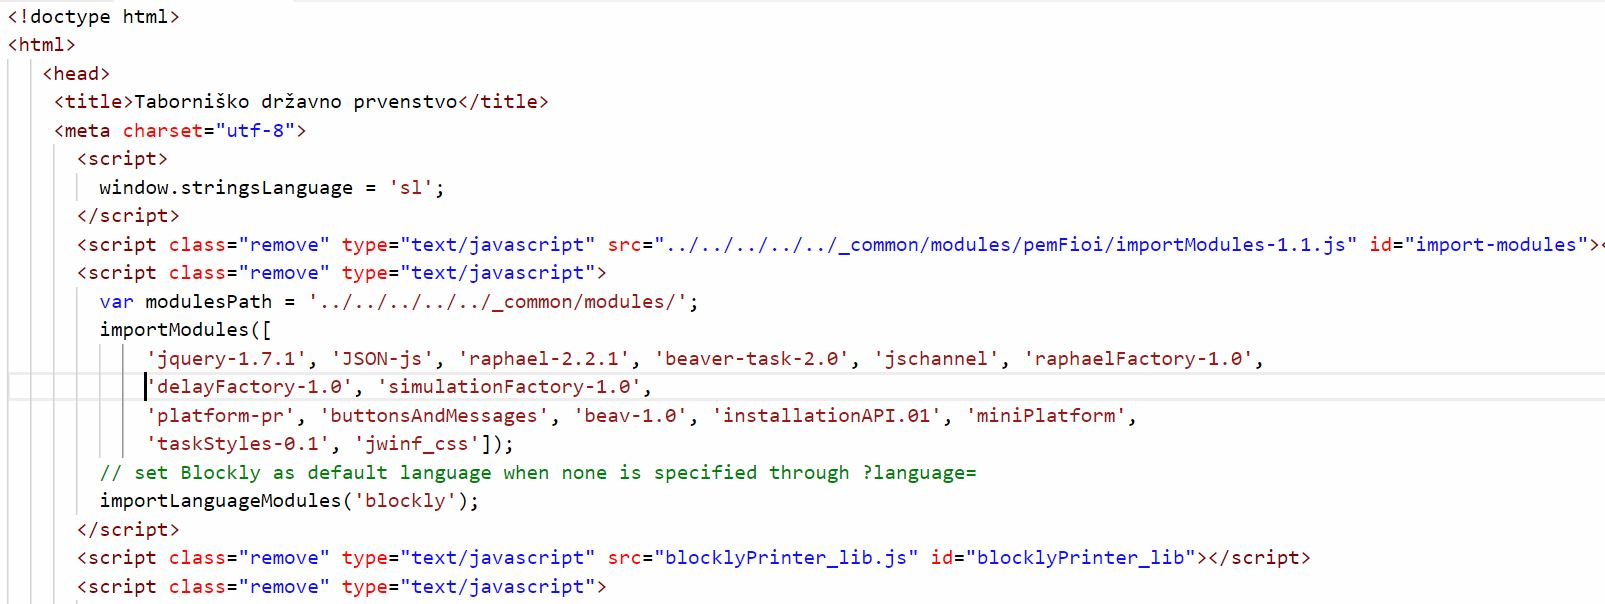
\includegraphics[scale=0.5]{index_splosno_zacetek}\\

Na začetku imamo naslov naloge (to ni dejansko naslov naloge temveč le ime, ki bo pisalo v zavihku v brskalniku), nato določimo jezik samega okna. V naslednjih vrsticah najprej uvozimo modul: \textit{importModules-1.1.js} oziroma katerokoli višjo/nižjo različico modulov. To je potrebno za samo lokalno testiranje delovanja našega programa. \\[0.5cm]
Pri uvažanju modula importModules-1.0 naloga dela na strežniku, vendar ne upošteva lokalne knjižnice blocklyRobot\textunderscore lib.js. Če pa se uporabi imporModules-1.1. naloga upošteva lokalno knjižnico, vendar ne dela na strežniku.\\[0.5cm]
\textbf{Zelo pomembno pri teh naslovih je kako nizko v drevesni strukturi se nahajamo, saj je od tega odvisno število "../" pred samim naslovom, prav tako je potrebno to, da na enak način spremenimo spremenljivko modulesPath, v naslednji vrstici.}\\[0.5cm]
Če teh nastavitev ne nastavimo pravilno se nam na lokalno naloga in sam index.html ne bo pravilno izpisal.
Nato uvozimo še datoteko textit{blocklyPrinter\textunderscore lib.js} oziroma ustrezno poimenovano datoteko glede na tip naloge in samega junaka.       \\[0.5cm]

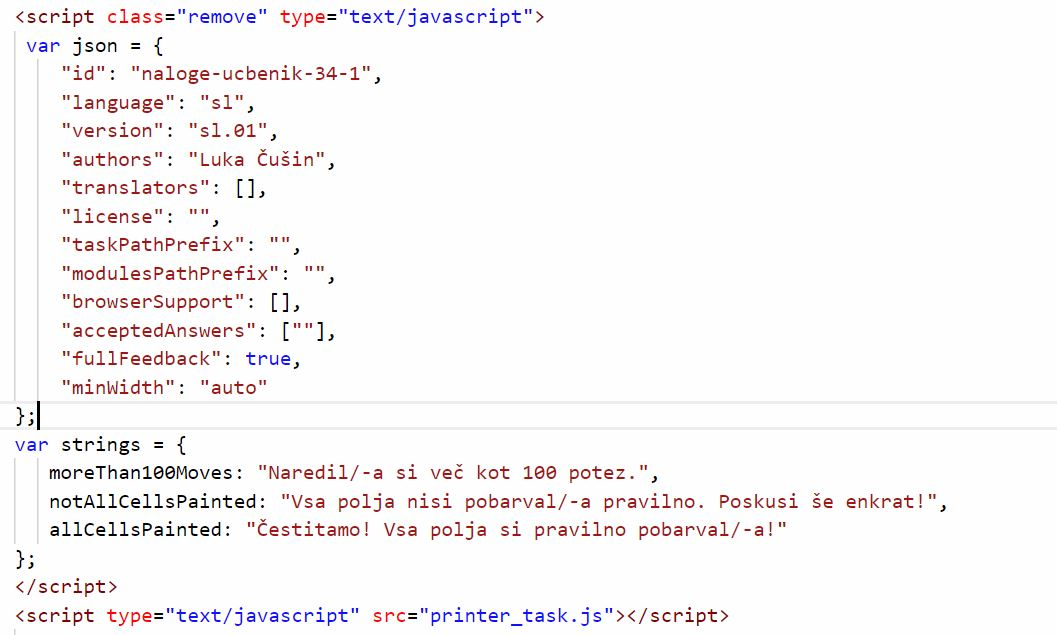
\includegraphics[scale=0.6]{index_splosno_json_spremenljivka}\\

V spremenljivko \textit{json} shranimo podatke, kot so avtor naloge, jezik naloge in nekatere druge podatke, kot so \textit{fullFeedback} ipd. \\
V spremenljivko \textit{strings} shranimo nekatere splošne podatke.

Dodamo fotografije, ki jih bomo uporabljali:\\
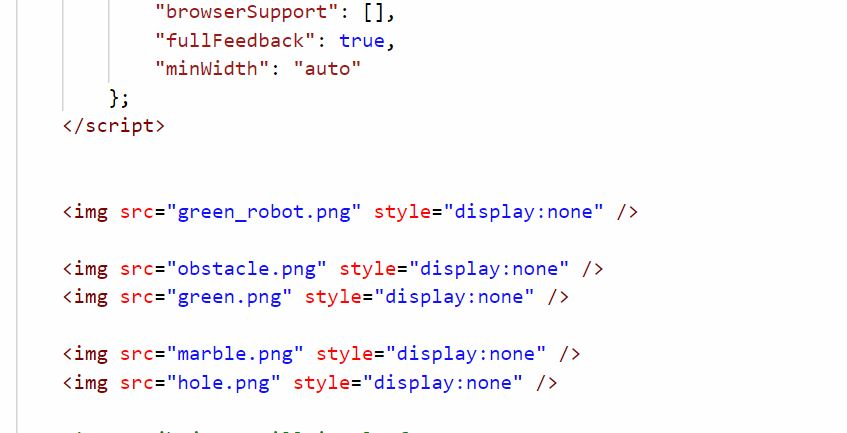
\includegraphics[scale=0.6]{index_foto_uvoz}\\
Na koncu samega \textit{head}-a pa uvozimo še ustrezno javascript datoteko, katere ime je prav tako odvisno od tipa naloge. \\

Če želimo dodati \textbf{namig} v nalogo, ga dodamo na tem mestu: \\

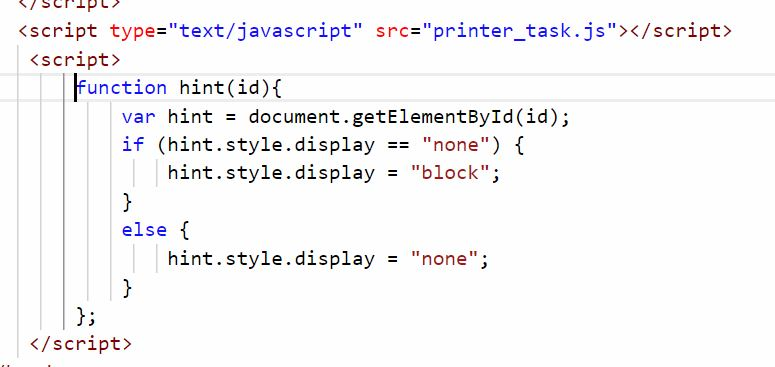
\includegraphics[scale=0.6]{index_splosno_hint_task}\\


Tu pa se začne dejansko besedilo vsake od nalog: \\

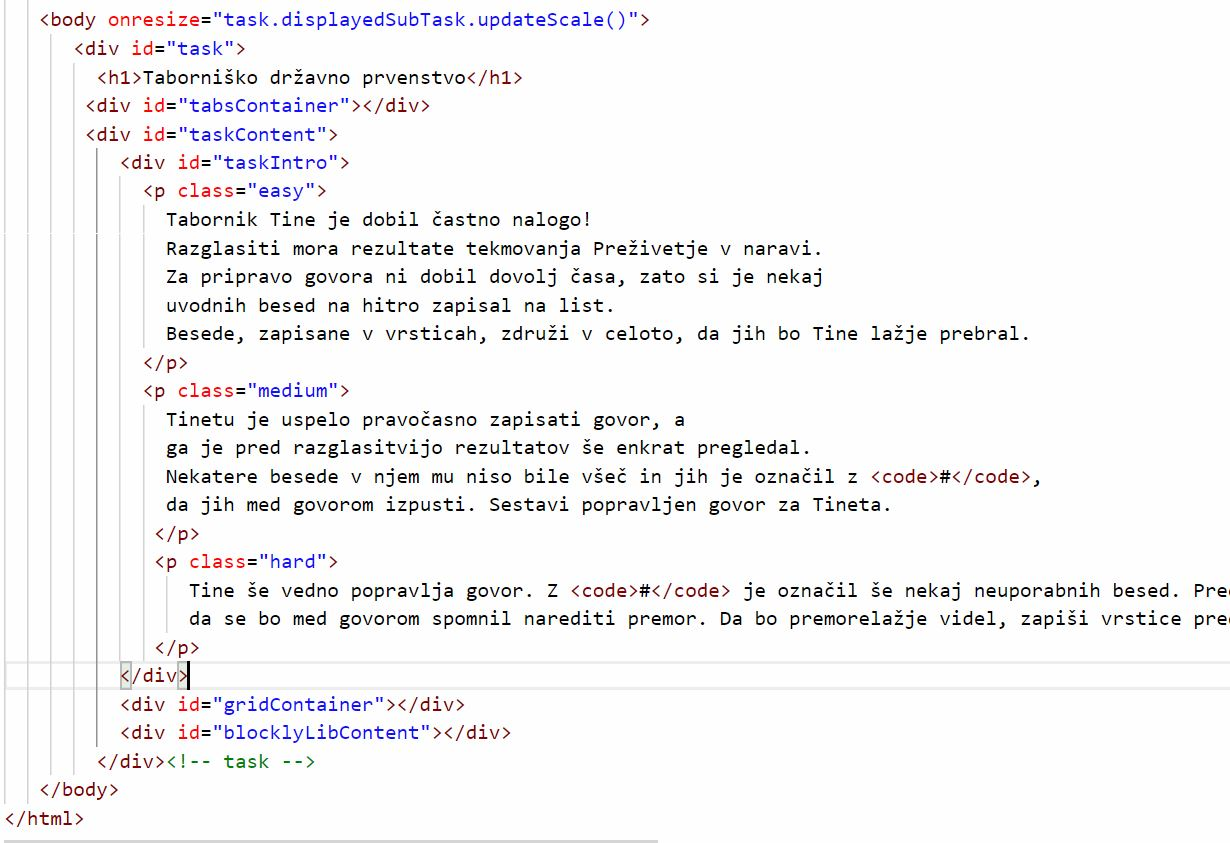
\includegraphics[scale=0.6]{index_splosno_body}\\

V tem delu definiramo kakšnega tipa je naloga, poznamo naslednje težavnosti:

\begin{itemize}
\item easy
\item medium
\item hard
\end{itemize}

Od tega je tudi odvisno koliko zvezdic se bo pokazalo v zgornjem zavihku.\\
Znotraj teh odstavkov pa stavimo dejansko navodilo naloge, ki je potem vidno uporabniku. \\
V primeru da teh tipov ne definiramo a vseeno imamo več podnalog, se besedilo prikaže pri vseh podnalogah, kot kaže spodnja fotografija.

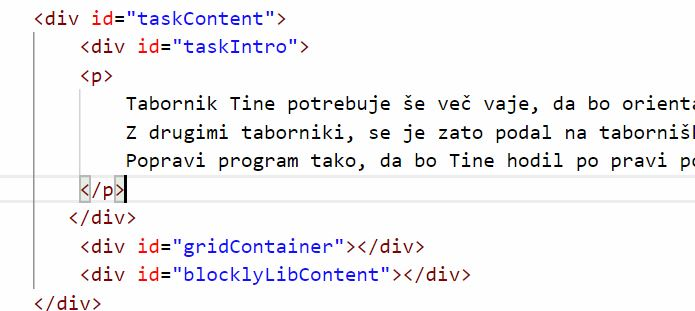
\includegraphics[scale=0.6]{index_ni_stopenj}
%%%%%%%%%%%%%%%%%%%%%%%%%%%%%%%%%%%%%%%%%%%%%%%%%%%%%%%%%%%%%%%%%%%%%%%%%%%%%%%%%%%%%%%%%%%%%%%%%%%%%%%%%%%%%%%%%TASK-SPLOŠNO
\subsubsection{task}

V tej datoteki, nastavimo parametre samega dela naloge, v kodo vstavimo že obstoječe bloke, nastavimo omejitve števila blokov, ustvarimo teste, ki bodo preverjali pravilnost našega programa, ipd. \\

Koda se začne z definicijo same funkcije: \\

\includegraphics[scale=0.6]{task_splosno_funkcija}\\

Nato se začne del, v katerem določimo lastnosti samega Blockly okolja. \\
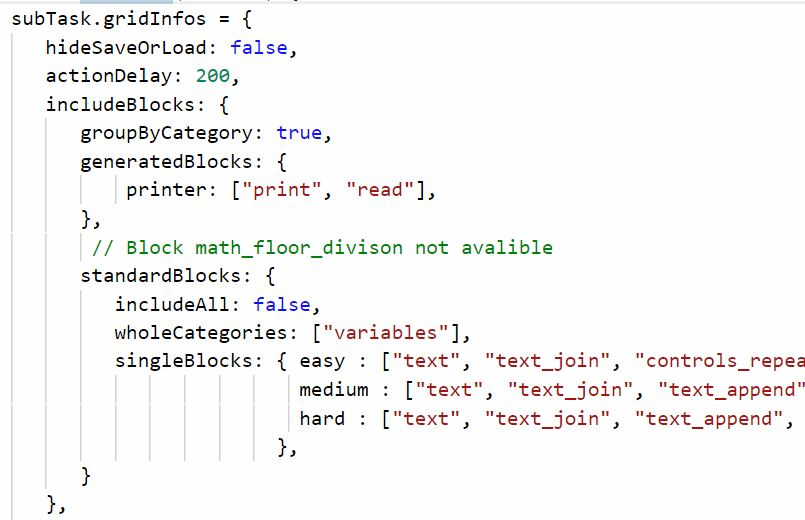
\includegraphics[scale=0.6]{task_splosno_grid_infos}\\

Tu določimo naslednje lastnosti:
\begin{itemize}
\item hideSaveOrLoad: false $\rightarrow$ kar pomeni, da se bo prikazal gumb, kjer lahko shranimo kodo ali jo kopiramo. \\

\includegraphics[scale=0.6]{nalozi,shrani}\\
\item \textbf{actionDelay: 200} $\rightarrow$ ki ob kliku za določen čas v milisekundah ustavi delovanje funkcije
\item \textbf{includeBlocks:}  $\rightarrow$ v katerem definiramo, da so bloki grupirani v skupine, ter katere bloke zgenerira.\\
\textbf{Tukaj je seznam kratic za vse standardne bloke katerih kratice je potrebno poznati, 
  ce želimo v nalogo dodati eno specificno kocko:}\\
		
		 \textit{https://gist.github.com/davidferguson/f85e1ae84b940bf8398f9bdbe98a4d8f}\\[0.5cm]

\item \textbf{standardBlocks:}  $\rightarrow$ v katerem lahko nastavimo, da ne vključi vseh blokov, nastavimo, da je vidna celotna skupina ipd.
\item \textbf{maxInstructions: (easy: 0, medium: 0, hard: 10)} $\rightarrow$ kar pomeni število dovoljenih blokov, ki jih uporabnik lahko uporabi. v primeru, da je število blokov 0, to pomeni, da omejitev števila blokov ni.
\item \textbf{checkEndEveryTurn: false} $\rightarrow$ kar pomeni, da je preverjanje na vsakem koraku izklopljeno, kar pomeni, da preverja samo končno situacijo.
\item \textbf{blocklyColourTheme: "bwinf"} $\rightarrow$ Pomeni, da uporablja eno od blockly-ijevih tem.
\item \textbf{checkEndCondition: function(context, lastTurn)} $\rightarrow$ je klic funkcije, ki preverja pravilnost programa $\rightarrow$ ta funkcija se nahaja v \textit{blocklyTabornik\textunderscore lib.js} oziroma v korespondentno poimenovani datoteki glede na samo tematiko. \\
\textbf{V tem delu lahko definiramo popolnoma svoje teste.}
\item \textbf{computeGrade: function(context, message)} $\rightarrow$ je funkcija, ki izračuna oceno kakšen procent rešitve je uporabnik pravilno naredil.
\end{itemize}


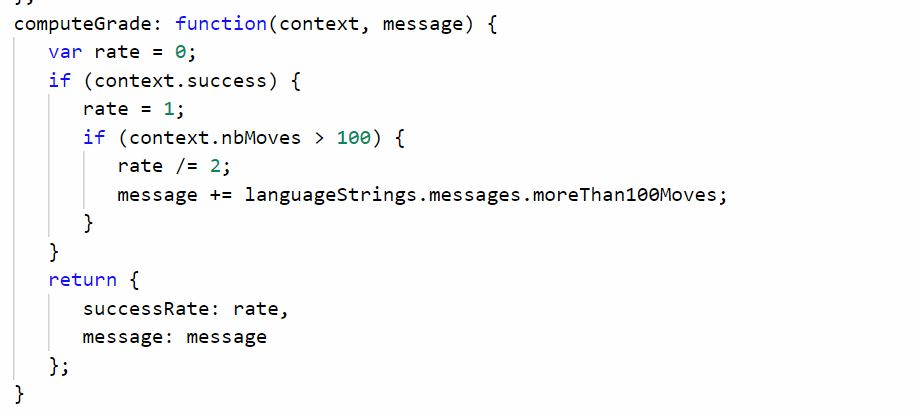
\includegraphics[scale=0.5] {task_vhod_compute_grade}

Nato pridemo do naslednjega dela, ki ga imenujemo \textit{data}, pri katerem napišemo lastnosti posameznih težavnosti. Ta del je razdeljen enako kot so razdeljena navodila v pripadajočem \textit{index.html}. \\
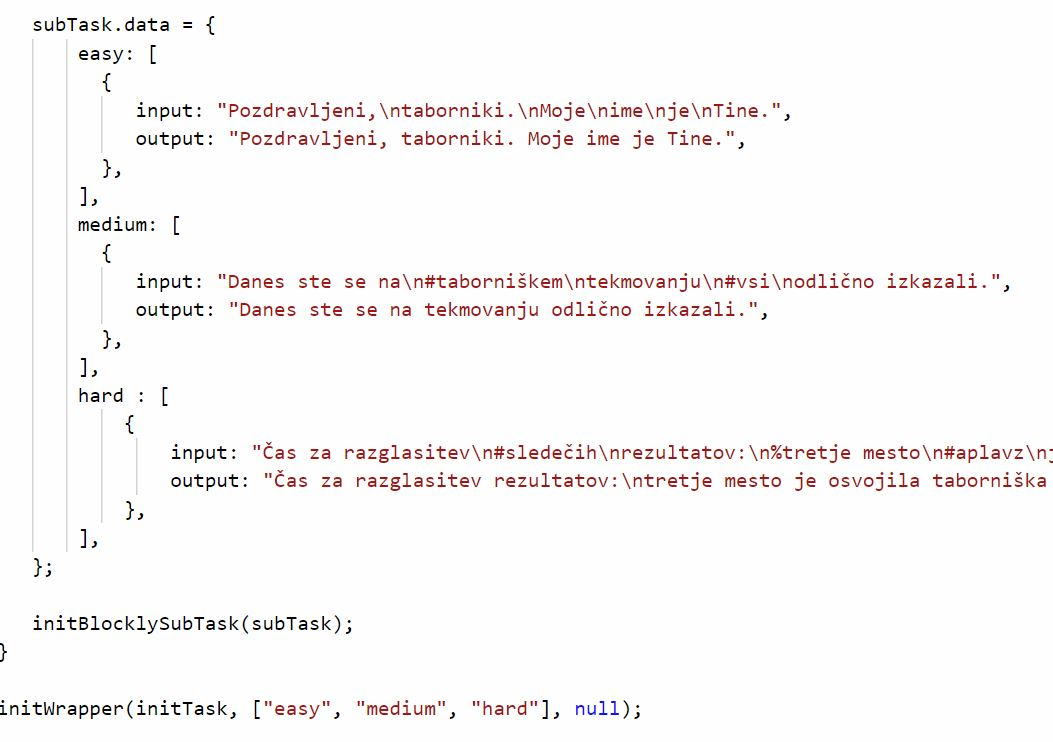
\includegraphics[scale=0.6]{task_splosno_data}\\

\textbf{V primeru, da želimo postaviti več različnih testov, lahko znotraj posamezne težavnosti (torej, easy/medium/hard), podamo več različnih testov, kot kaže spodnja fotografija.}\\

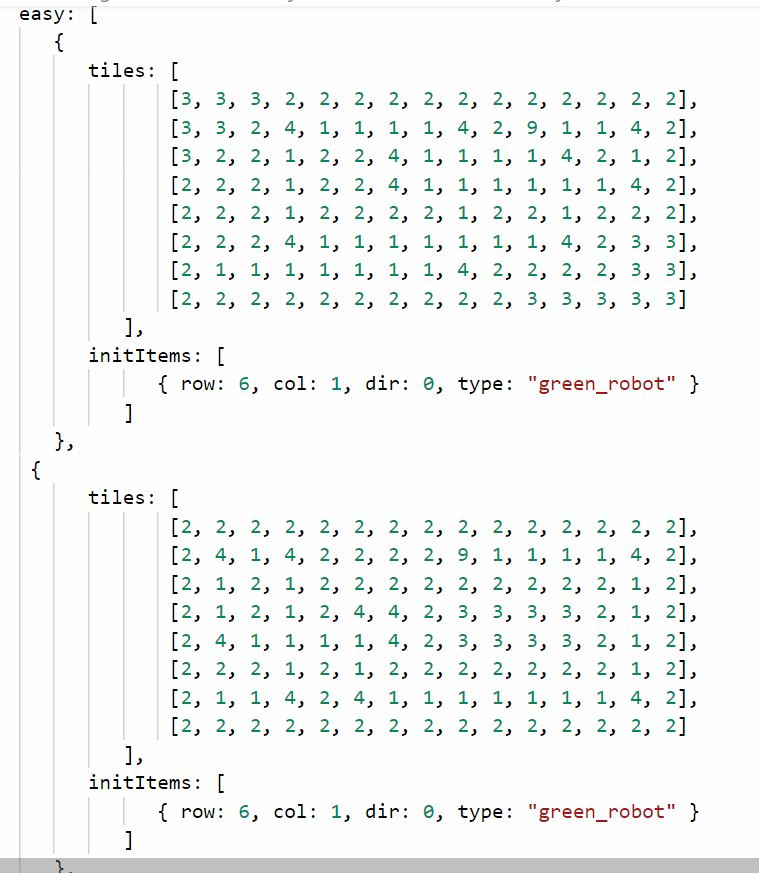
\includegraphics[scale=0.4]{task_splosno_data_vec_testov}

Na koncu v oglatih oklepajih v \textit{initWrapper} dodamo to funkcijo initTask, težavnosti, ki jih imamo, ter \textit{null}.
%______________________________________________________________________________________________________________________MREŽA___%%%%%%%%%%%%%%%%%%%%%%%%%%%%%%%%%%%%%%%%%%%%%%
\subsection{Mreža}

To so naloge, pri katerih se junak/več junakov premika po mreži. 
\subsubsection{task}
\begin{itemize}
\item \textbf{cellSide} $\rightarrow$ ki nastavi velikost enega kvadratka mreže (oziroma velikost mreže)
\item \textbf{backgroundColor} $\rightarrow$ spremenljivka določa barvo polj (barva zapisana v HEX)
\item \textbf{borderColor} $\rightarrow$ spremenljivka določa barvo roba polj (barva zapisana v HEX)
\item \textbf{noBorder} $\rightarrow$ izberemo ali črte med kvadratki narišemo
\end{itemize}
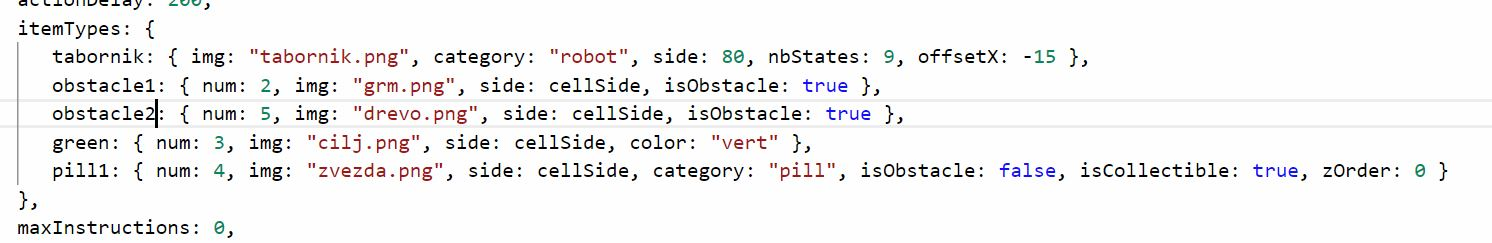
\includegraphics[scale=0.6]{mreza_task_tipi}\\
Te tipi imajo naslednje lastnosti:\\ (odvisno je tudi od tega kakšnega tipa je objekt)
\begin{itemize}
\item \textbf{img}  $\rightarrow$ ki se navezuje na fotografijo, ki je bila definirana v index-u ter se nahaja na istem direktoriju kot ta \textit{javascript} datoteka.
\item \textbf{category}  $\rightarrow$ ki se nanaša na to katere kategorije je objekt
\item \textbf{num}  $\rightarrow$ ki definira številko objekta, ki jo potem uporabi pri testih.
\item \textbf{side}  $\rightarrow$ ki pove kakšna je velikost kvadratka.
\item \textbf{isObsticle}  $\rightarrow$ ki pove če je objekt ovira ali ne
\item \textbf{isCollectable}  $\rightarrow$ ki pove, če se objekt lahko pobere
\item \textbf{zOrder}  $\rightarrow$ ki nam pove orientacijo v prostoru, kateri predmet bo pred drugim
\item \textbf{nbStates}  $\rightarrow$ število zazličnih pozicij, ki jih lahko ta objekt ima, torej vključuje rotacije ipd.
\item \textbf{offsetX}  $\rightarrow$ ki zamakne objekt v x-osi.
\end{itemize}

Obstajajo tudi drugi parametri, ki si jih lahko pogledate tukaj:\\
\textit{https://github.com/France-ioi/bebras-modules/tree/master/pemFioi/quickAlgo}.

Pri tipu naloge \textit{mreža} je \textit{data} definiran tako, da definiramo:\\
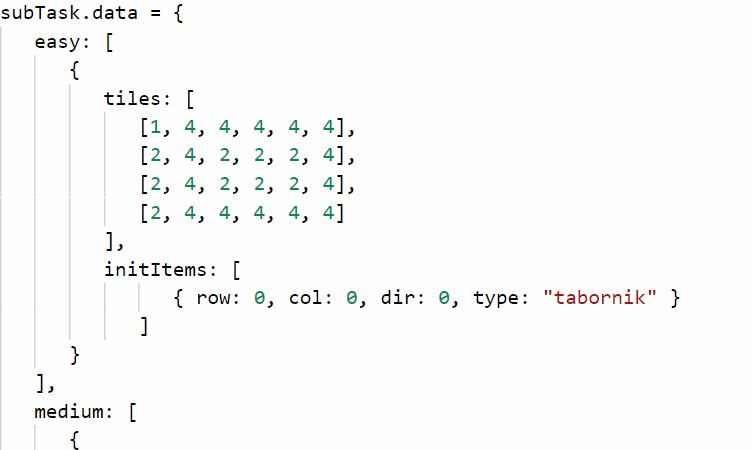
\includegraphics[scale=0.5]{mreza_data}\\
\begin{itemize}
\item \textbf{tiles}  $\rightarrow$ ki predstavlja tabelo številke v njej pa se nanašajo na številke fotografij definirane zgoraj v tipih objektov, številka 1 pomeni da je polje prazno \textbf{(na tem mestu ne definiramo premikajočih se elementov)}.
\item \textbf{initItems}  $\rightarrow$ kjer nastavimo zečetno pozicijo našega/naših junakov, v primeru da jih je več, jih naštejemo več.\\
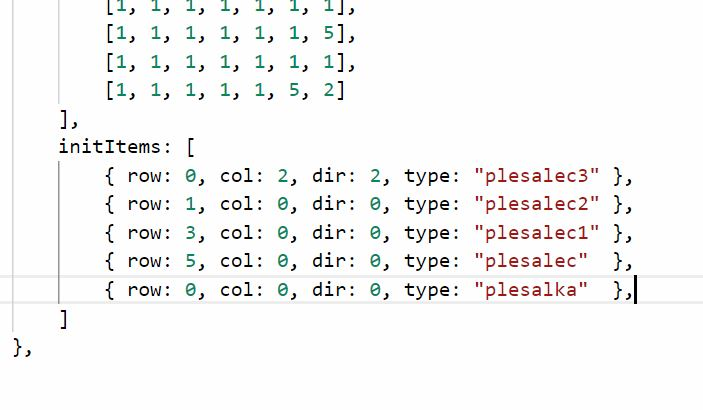
\includegraphics[scale=0.5]{mreza_vec_elementov}
\end{itemize}
%______________________________________________________________________________________________________________________ŽELVA___%%%%%%%%%%%%%%%%%%%%%%%%%%%%%%%%%%%%%%%%%%%%%%
\subsection{Risanje}

Pri tem tipu naloge gre za risanje nekega junaka na platno.

\subsubsection{task}

najprej v \textit{generatedBlocks} vstavimo definirane bloke.\\
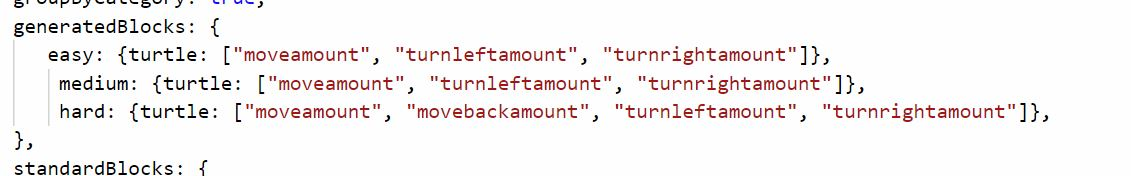
\includegraphics[scale=0.5]{risanje_generirani_bloki} \\
Nastavimo korak junaka:\\

\includegraphics[scale=0.5]{risanje_step_size_coords} \\
Lastnost \textit{coords} premakne celotno fotografijo.

V Preverjanje pravilnosti programe torej v \textit{checkEndCondition} napišemo funkcijo, ki jo definiramo v ali kar v \textit{task.js} ali pa v korespondenčni knjižnici, v našem primeru v \textit{blocklyTurtle\textunderscore lib}.
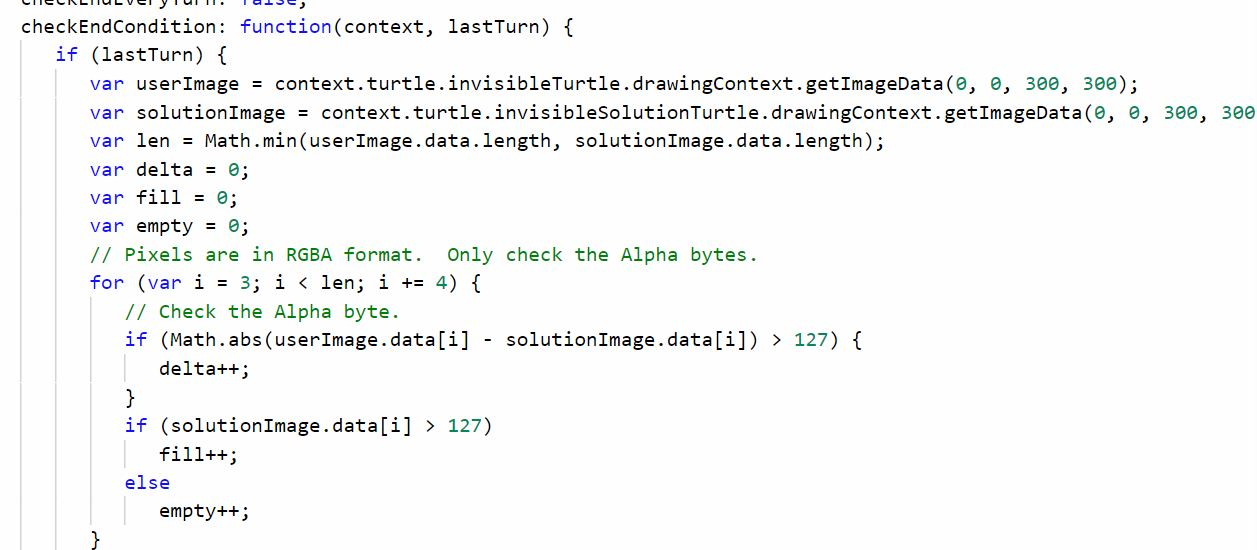
\includegraphics[scale=0.5]{risanje_check_end_condition} \\

\textit{Data} je lahko definiran tako:\\
%%%%%%%%%%%%%%%%%%%%%%%%%%%%%%%%%%%%%%%%%%KAKO NE POKAZATI PRAVILNE REŠITVE?%%%%%%%%%%%%%%%%%%%%%%%%%%%%%%%%%%%%%%%%%%%
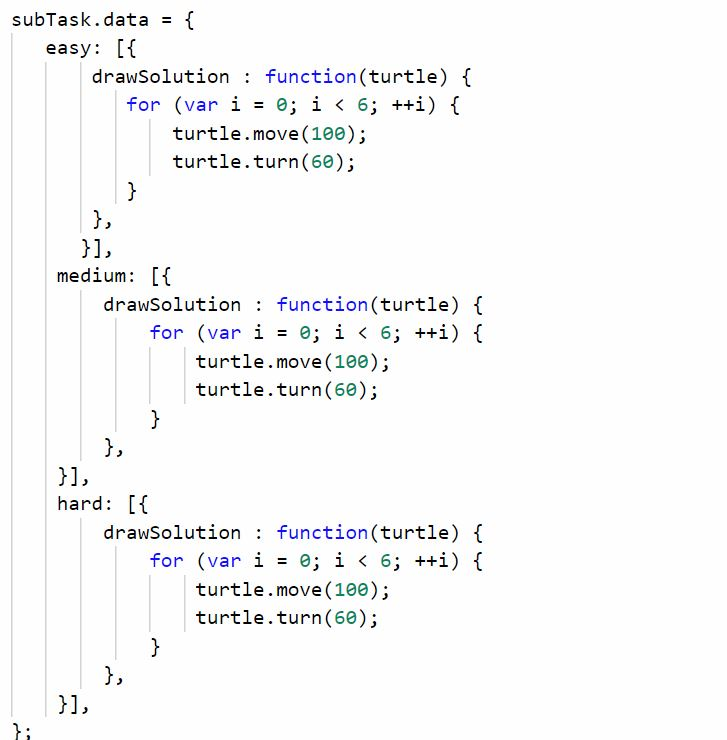
\includegraphics[scale=0.5]{risanje_task_data} \\

Kjer v premenljivko \textit{drawSolution} shranimo pravilno rešitev.
%______________________________________________________________________________________________________________________VHOD/IZHOD___%%%%%%%%%%%%%%%%%%%%%%%%%%%%%%%%%%%%%%%%%%%%
\subsection{Vhod/izhod}

To so naloge, pri katerih je potrebno napisati nekaj v okno. ta rezultat se preveri.
\subsubsection{task}
 Naloge delujejo tako, da skozi spremenljivki \textit{input} in \textit{output} dodamo kako naj bi izgledala naloga in kaj bi bila pravilna rešitev. \\
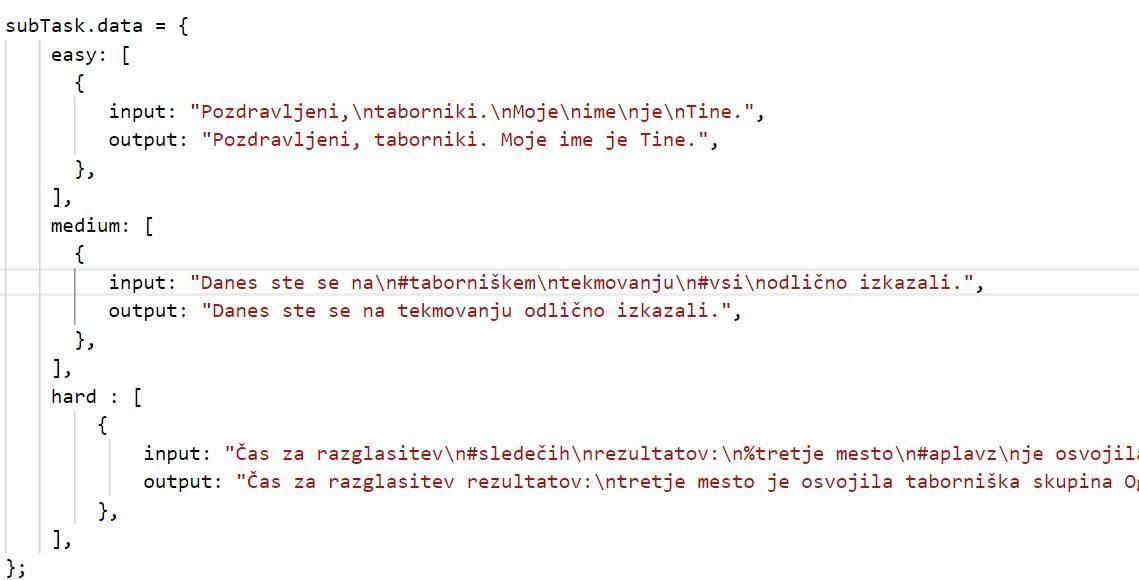
\includegraphics[scale=0.6]{task_vhod_data}\\


\pagebreak

%______________________________________________________________________________________________________________________Spicifični sklopi___%%%%%%%%%%%%%%%%%%%%%%%%%%%%%%%%%%%%%%%%%%%%
\subsection{Specifični sklopi}

\subsubsection{Tabornik}
\begin{itemize}
\item Naloge sklopa Tabornik delujejo z modulom importModules-1.1., vendar samo ce se lokalna knjižnica nahaja v isti datoteki kot index.
\item
\end{itemize}
%__________________________________________________Administratorski vmesnik
\section{Administratorski vmesnik}

Administratorski vmesnik, se uporablja predvsem zato, da upravljalci nalog lahko konkretno testirajo, in upravljajo z objavljenimi nalogami.
Najprej je potrebno navigirati na:\\
\begin{center}
\textit{http://pisek.acm.si/admin/index.html}
\end{center}
Nato vpišete naslednje uporabniško ime in geslo:
\begin{center}
\textit{Uporabniško ime: } pronal\\
\textit{geslo: } pronal\textunderscore pisek\\
\end{center}
Ko ste prijavljeni, lahko na levi strani vidite drevesno strukturo, na desni strani pa so različni zavihki, v katerih lahko urejate različne sklope/naloge ipd.\\
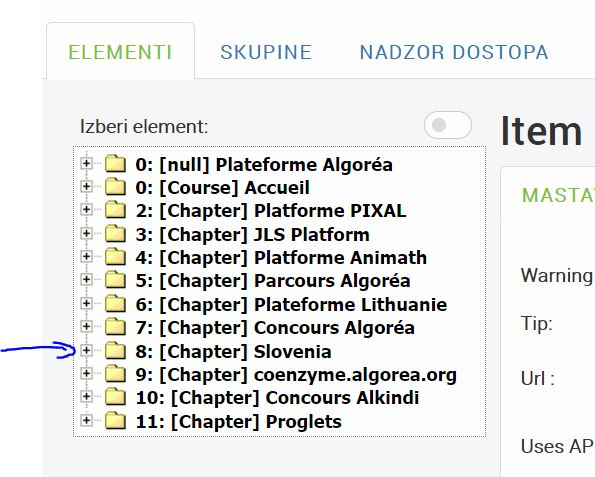
\includegraphics[scale=0.8]{admin_drevo}\\

Naloge se nahajajo v mapi slovenija, ter znotraj podmape \textit{Učna pot}. \\
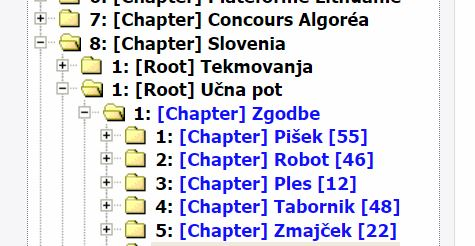
\includegraphics[scale=0.8]{admin_drevo_odprto}\\

\pagebreak
Znotraj Piška poznamo dva tipa, tip \textit{Chapter} in tip \textit{Task}. Prvi tip predstavlja mapo, v kateri so naloge, drugi tip predstavlja dejansko nalogo.\\

\includegraphics[scale=0.7]{zmajcek_task}

Na desni strani, so v zavihkih različne funkcije, ki se nanašajo predvsem na lastnosti naloge oziroma sklopa, torej:
\begin{itemize}
\item Dejanski URL naloge, ki ga nastavimo pri uvozu naloge.\\
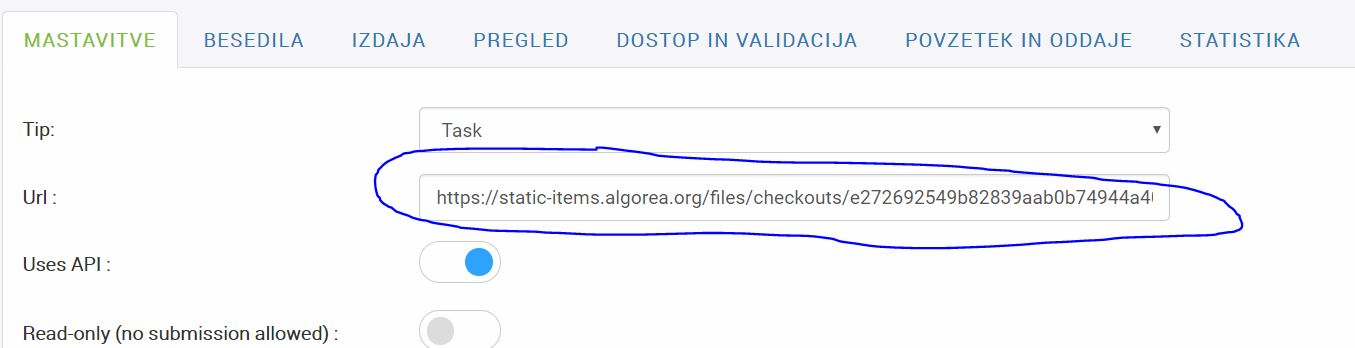
\includegraphics[scale=0.7]{task_url}
\item Validacija naloge, ki nalogo naredi skrito oziroma odprto.\\
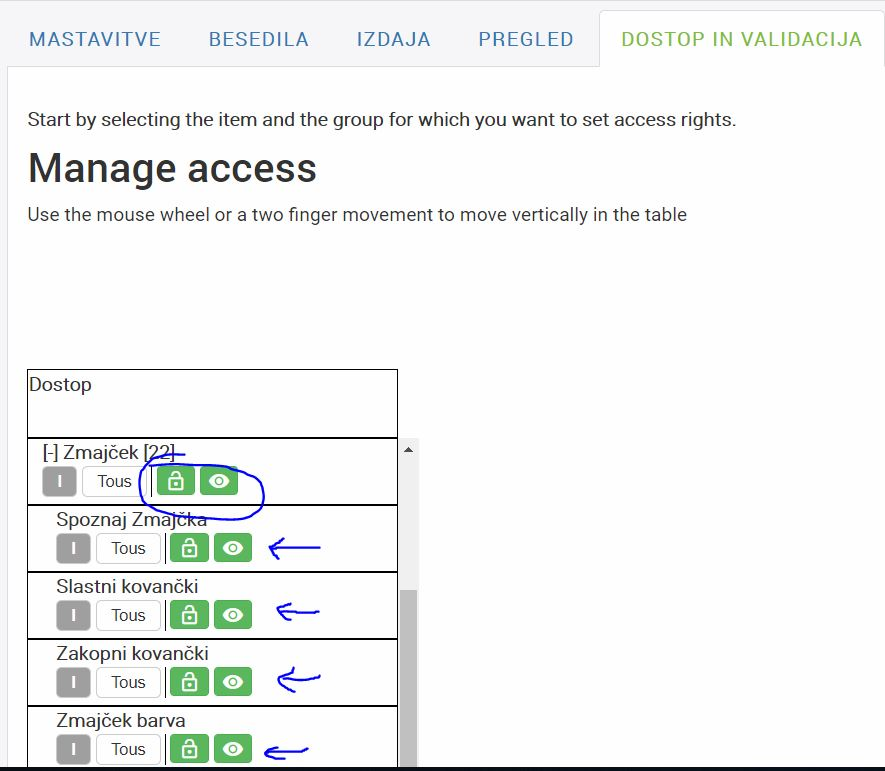
\includegraphics[scale=0.4]{validacija_admin}
\pagebreak
\item Naslov naloge/sklopa ter opis sklopa\\
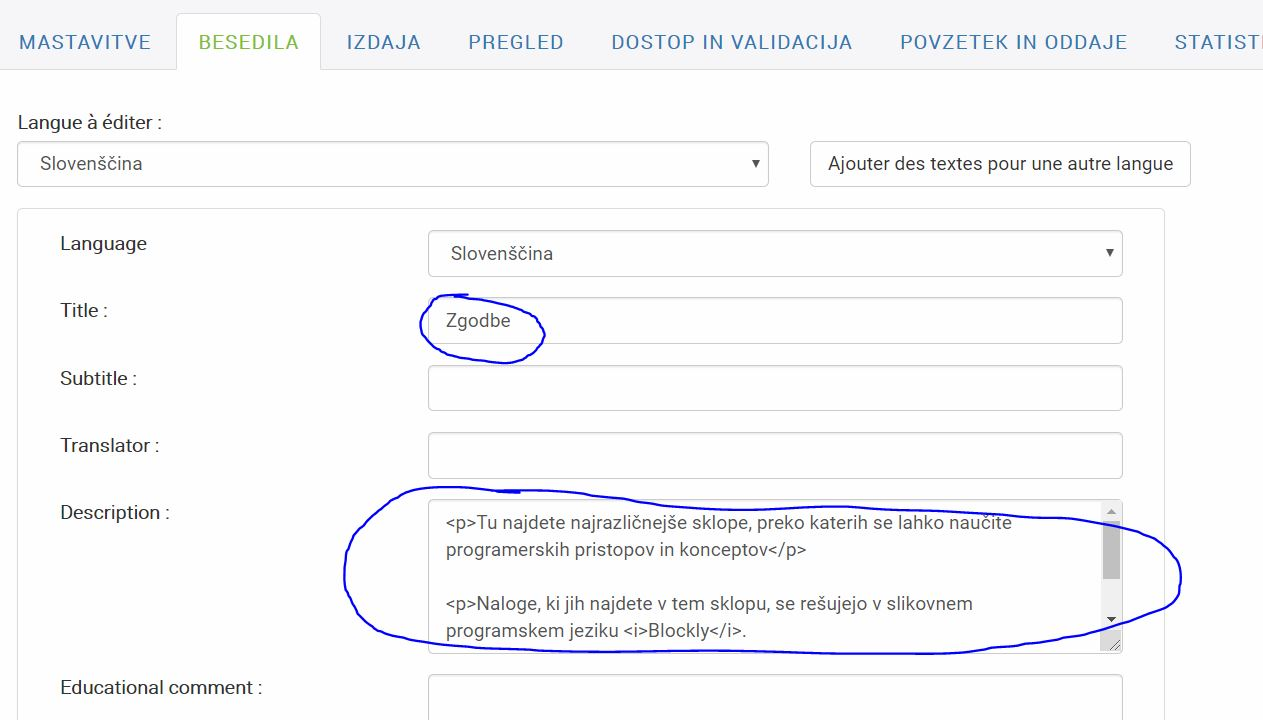
\includegraphics[scale=0.4]{naslov_besedilo}
\end{itemize}

V sami drevesni strukturi, lahko naloge/sklope tudi kopiramo ali jih izbrišemo (desni klik), vendar moramo biti pri tem pozorni, saj je potrebno ločevati med tem da nalogo naložimo z drugačnim URL-jem na portal, ker se v primeru kopiranja, dejanski url prav tako kopira, kar pomeni, da če nalogo spremenimo in jo posodobimo na portalu, se bo naloga spremenila tudi na klonu naloge. V primeru da original izbrišemo, se klon ne izbriše.

Podobne modifikacije se da delati tudi na dejanskem Portalu Pišek, le z nekaterimi omejitvami.
Prijavno okno je bilo skrito (s strani Administratorjev strežnika - Za spremembo je potrebno kontaktirati le te)

povezava za samo prijavo pa se nahaja na tem naslovu:
\begin{center}
\textit{https://login.france-ioi.org/auth}
\end{center}
Geslo in uporabniško ime sta enaka, kot za administratorski vmesnik.
V samem administratorskem vmesniku so še nekatere dodatne funkcije/lastnosti nalog in sklopov, ki pa si jih poglejte sami.


\pagebreak
%__________________________________________________SVN
\section{SVN Repozitorij}

%_____________Vzpostavitev
\subsection{Vzpostavitev SVN repozitorija}
Za uspešno vzpostavitev repozitorija je potrebno imeti program, ki podpira SVN-repozitorija.
V našem primeru bomo uporabili \textbf{TurtioseSVN}.
Program lahko dobite na tem naslovu:\\
\begin{center}
\textit{https://tortoisesvn.net/downloads.html}\\
\end{center}

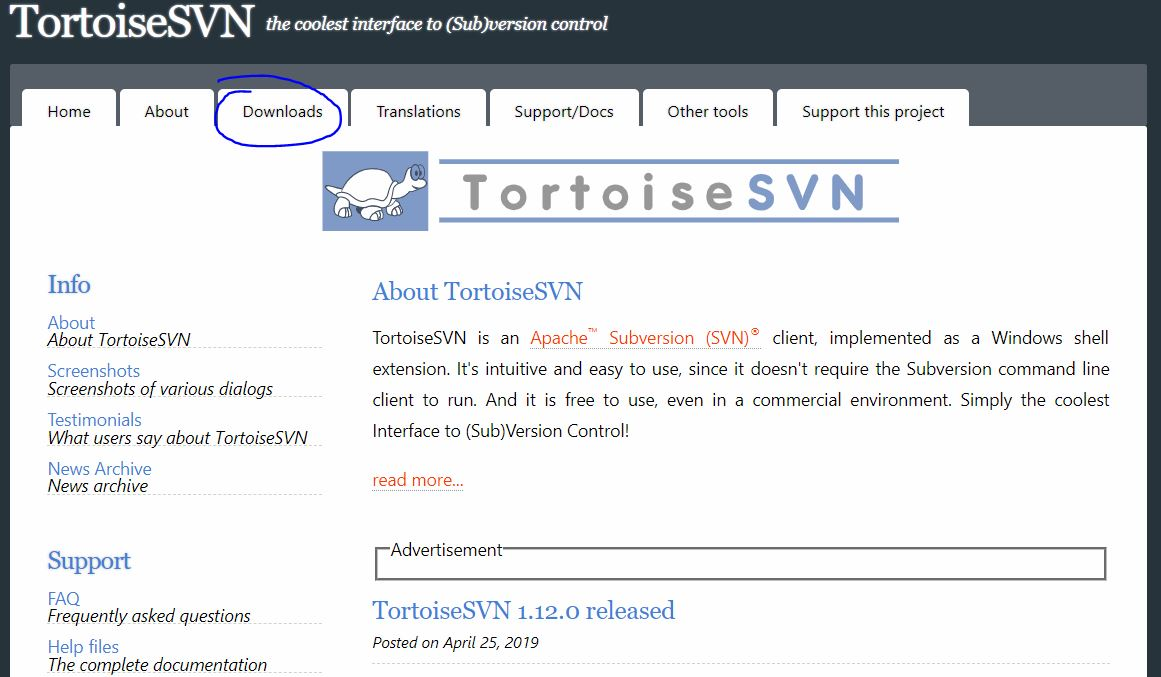
\includegraphics[scale=0.4]{turtoise_svn}\\

Ko je program naložen, lahko s pomočjo desnega klika na lokacijo, na katero želite vzpostaviti repozitorij izberete možnost \textit{SVN Checkout}.\\
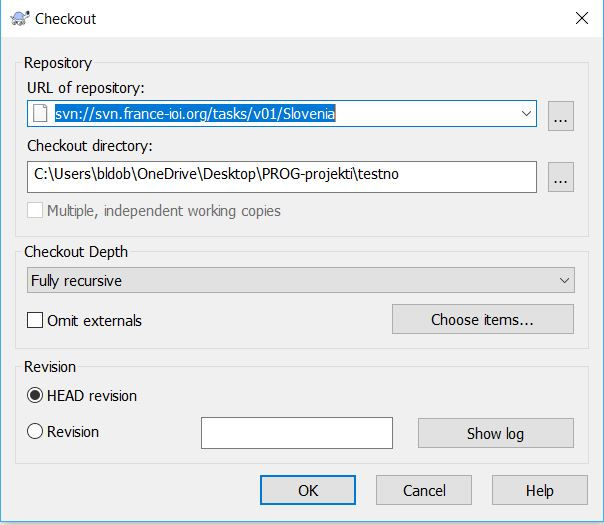
\includegraphics[scale=0.4]{svn_okno}\\

v URL of repository vpišemo naslenje:\\
\begin{center}
\textit{svn://svn.france-ioi.org/tasks/}
\end{center}

Ko kliknemo Ok, se prične nalaganje, ko se naložijo vse datoteke, ste vzpostavili SVN-repozitorij.\\
\pagebreak
%____________Struktura
\subsection{Struktura SVN repozitorija}
SVN je strukturiran tkao, da imamo najprej zunanjo mapo, ki je podobna kot pri administratorskem vmesniku, nato pa podobno kot tam navigiramo v mapo Slovenia.\\
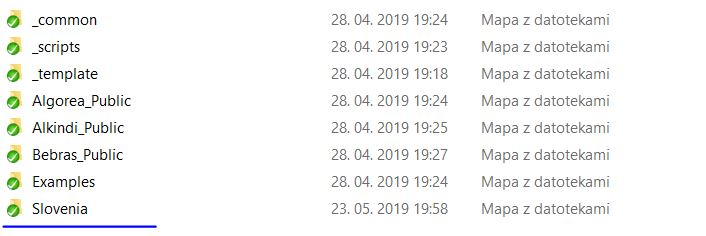
\includegraphics[scale=0.6]{svn_zunanja}\\

Kar se tiče drevesne strukture na SVN vmesniku, je tako, da je struktura postavljena kar se da podobno kot struktura na samem portalu.\\
\textbf{Natančneje:} \\[0.5cm]
Sklopa \textit{Zgodbe} in sklop \textit{Učbenik} sta sklopa, v katerih se nahajajo originalne naloge, medtem ko v  sklopih \textit{Navodila}, kjer se nahajajo ta navodila in vse datoteke za spreminjanje, navodil, \textit{CodeWeek}, kjer načeloma ni ničesar, razen, če se v prihodnosti na CodeWeek objavljajo originalne naloge, Na portalu, pa so večinoma naloge kopije nalog iz zgodb in učbenika. Enako velja za sklop \textit{Programski koncepti}. Kar se tiče ostalih map, so to mape, ki vključujejo različne module, ki so potrebni za uspešno izvajanje in lokalno testiranje.\\
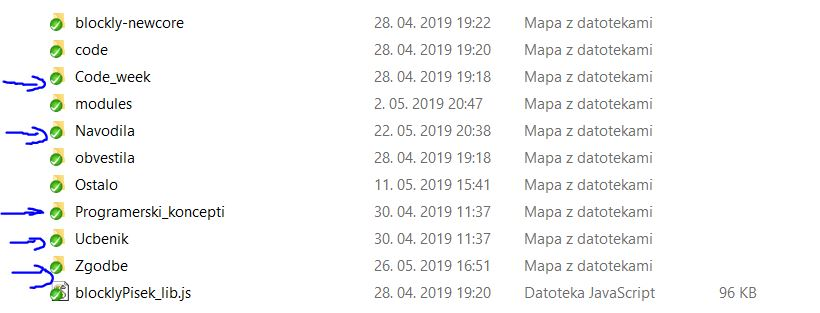
\includegraphics[scale=0.5]{svn_slovenia}


Vsebina posamezne naloge in pot izgleda približno takole:\\
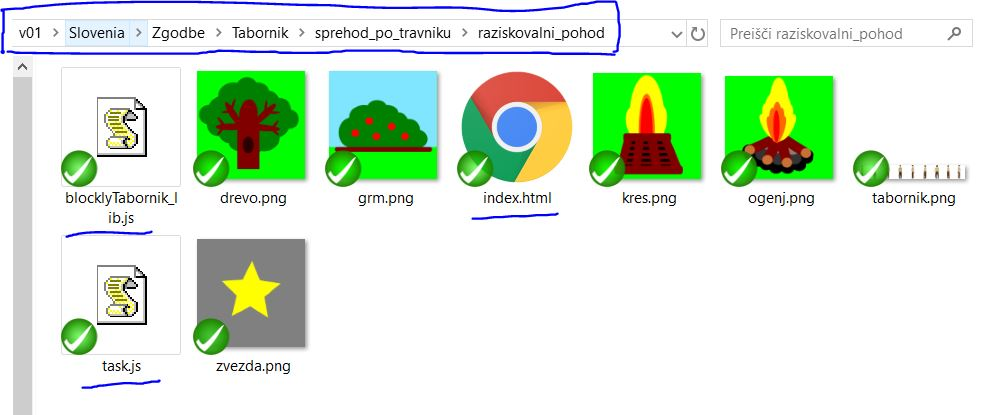
\includegraphics[scale=0.5]{svn_naloga}

Tudi pot je takšna, kot je pot na dejanskem portalu. To sicer pomeni več dela v primeru premikanja nalog, vendar se v večini od teh nalog nebi smela spreminjati naslov/pot. Kot je bilo opisano v sklopu Nove naloge so pomembne podčrtane datoteke.
\pagebreak
%__________Nalaganje
\subsection{Nalaganje na SVN repozitorij}
Naloge najlažje dodamo na SVN tako, da jih dejansko ustvarimo (oziroma kopiramo že obstoječo nalogo in jo preuredimo, tako, kot si jo želimo). Nato pa z desnim gumbom kliknemo na lokacijo SVN-repozitorija in izberemo možnost \textit{SVN Commit...}\\
Prikaže se nam tako okno: \\[0.5cm]
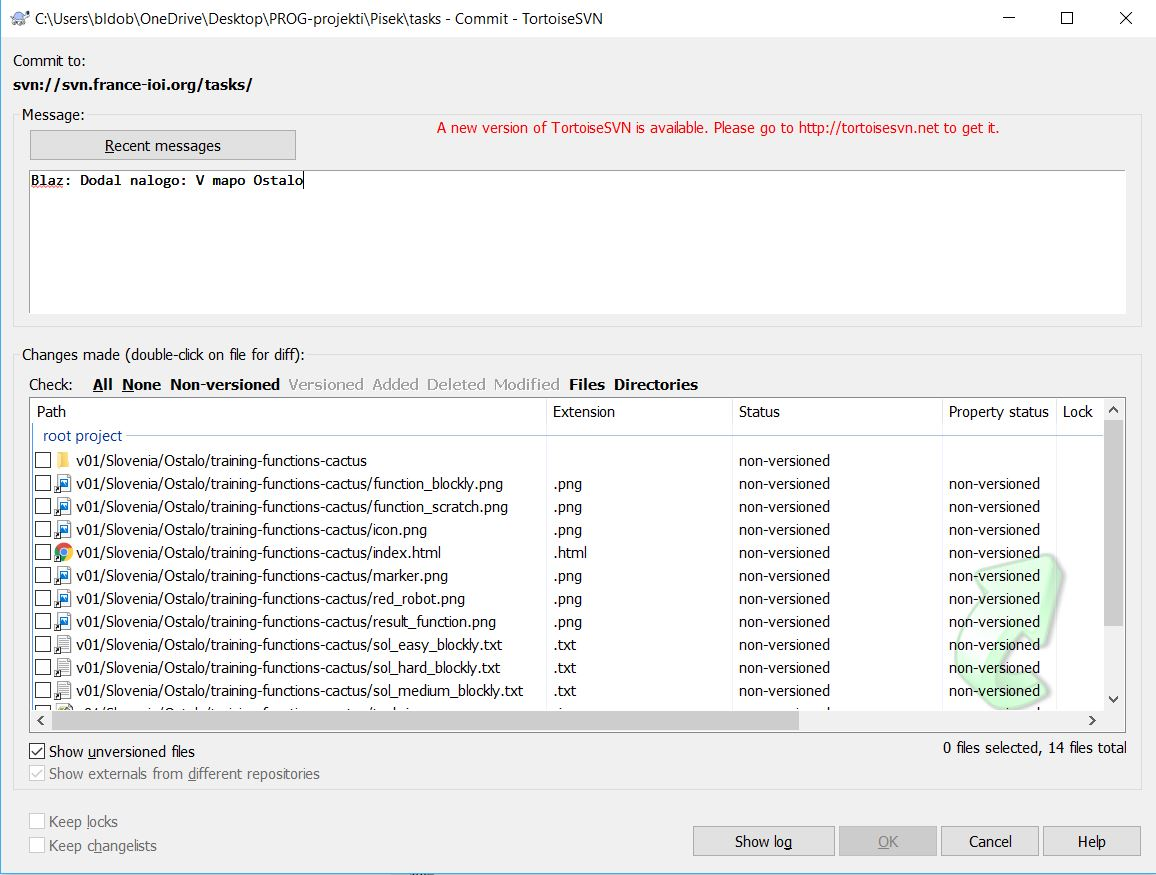
\includegraphics[scale=0.5]{svn_nalaganje}\\[0.5cm]
kjer napišemo sporočilo v obliki:\\
\begin{center}
\textit{IME: Sporočilo}
\end{center}
Izberemo datoteke, ki jih želimo naložiti na repozitorija in kliknemo OK. Naloga se naloži.

\pagebreak
%__________________________________________________Nalaganje na Portal Pišek
\section{Nalaganje na Portal Pišek}

Ko imamo nalogo na SVN repozitoriju, jo lahko impotiramo tudi na portal, to naredimo prek naslednje povezave:\\
\begin{center}
\textit{http://svnimport.france-ioi.org}
\end{center}

Potrebno je vpisati uporbniško ime in geslo:\\

\begin{center}
\textit{Uporabniško ime: }  jernej.vicic\\
\textit{geslo: } slov798xb2127x9ssX\\
\end{center}
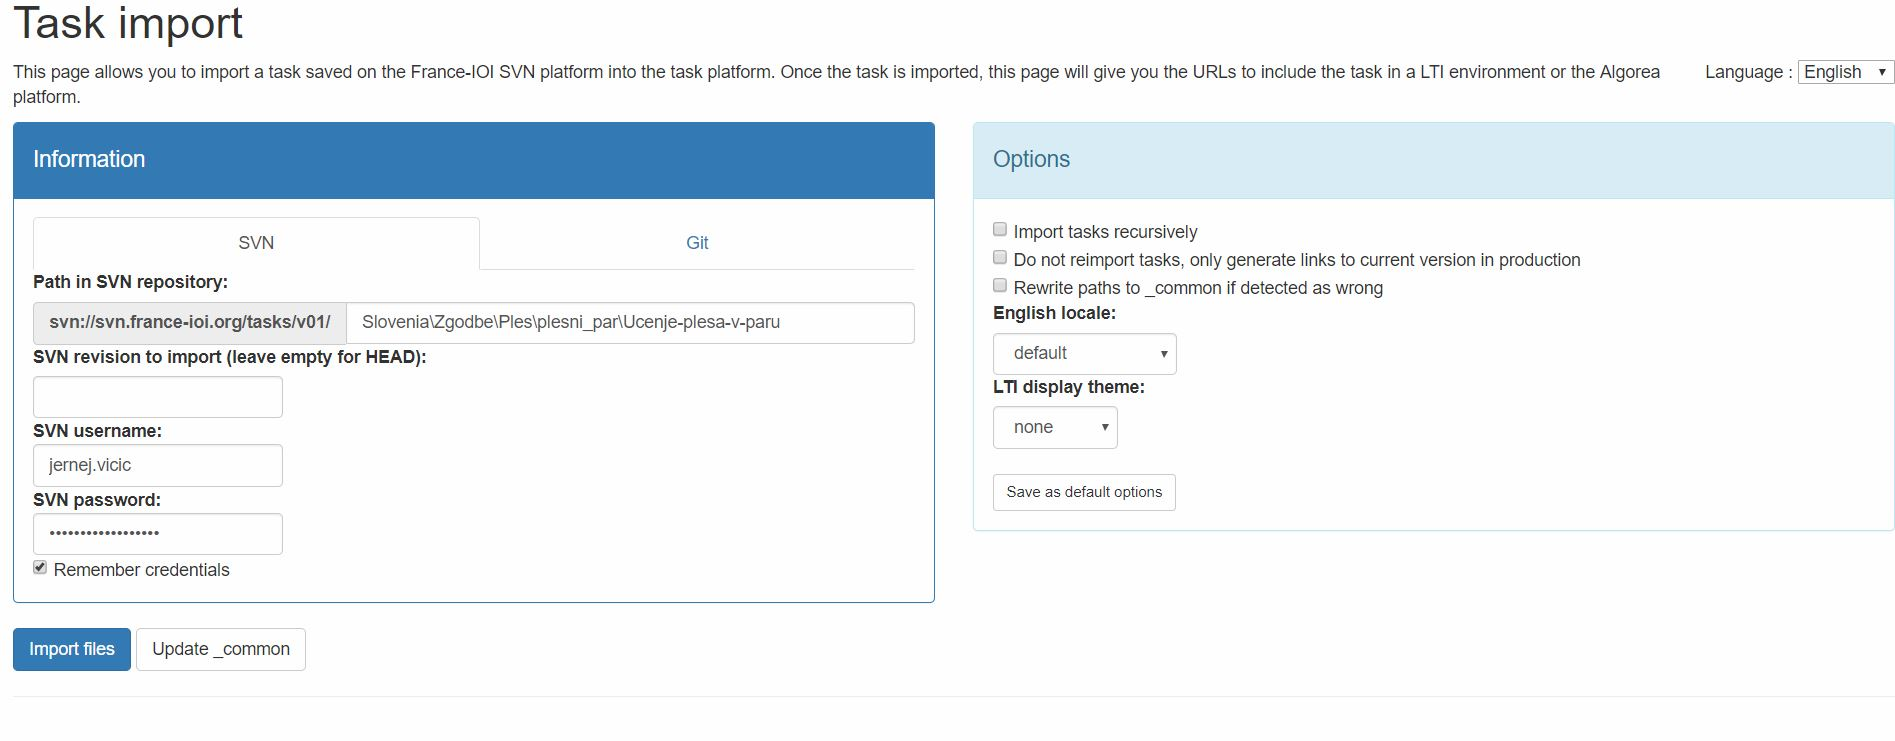
\includegraphics[scale=0.5]{objavljanje_nalog}\\[0.5cm]
Na ustrezna mesta vpišemo podatke, dodamo pot v SVN repozitoriju, kot je prikazano na zgodnji sliki.\\

Ko se naloga uvozi, se pojavi povezava, s katero dostopate do lokacije naloge.\\
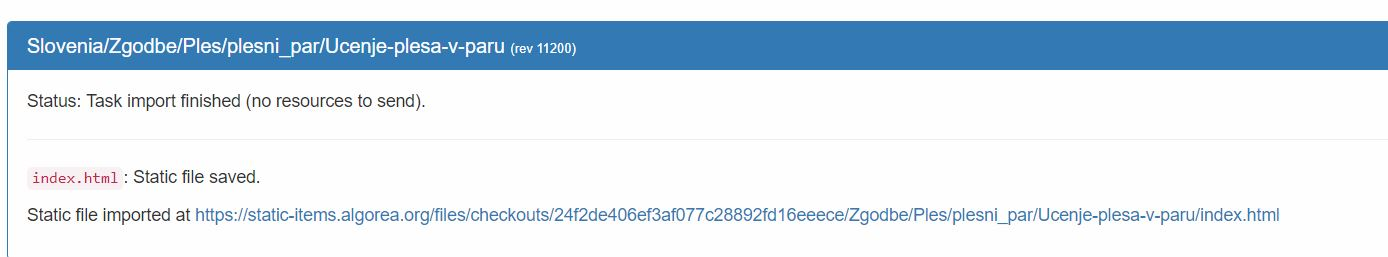
\includegraphics[scale=0.5]{povezava}\\[0.5cm]

\textbf{Če na SVN-ju ne spreminjamo drevesne strukture (in ne preimenujemo map) in posodabljamo datoteke (commitamo) in nalogo naložimo na strežnik, je naceloma dovolj samo osvežiti piškovo spletno stran, pa bi morala biti opazna razlika.}
V primeru  da se to ne zgodi, poskusite zbrisati zgodovino podatkov v vašem brskalniku.\\[0.5cm]

Nato v novem zavihku navigirate na administratorski vmesnik, ki se nahaja tukaj: 

\begin{center}
\textit{http://pisek.acm.si/admin/index.html}
\end{center}

Kliknite na ustrezno željeno mesto v drevesni stukturi z desnim klikom se vam pokažejo možnosti, izberite možnost new. Na tak način ustvarite enoto. Če izberete tip "Chapter" ustvarite imenik, če pa "Task" pa nalogo. Tako lahko ustvarimo poljubno drevesno strukturo in vanjo uvrstimo
naloge.\\

Za nalogo je dovolj nastaviti le URL, pravilen tip in vklopiti "Uses API" (ki
je privzeto vklopljen).



\end{document}
